\section{Reasoning Framework Overview\label{sec:framework}}

The design goals of our framework are modularity for the
transformation steps and flexibility with respect to the
underlying inference engine. The high modularity allows to reuse
transformation functionality across different WSML variants and
reduces the effort for accomplishing other reasoning tasks. By
reducing WSML to simple Datalog constructs and providing a
respective object model we have reduced the effort of integrating
new reasoners to a minimum\footnote{In fact, the adaptation of the
framework to the MINS rule engine took less then a day.}. The
presented framework has been implemented in Java and can be
downloaded at {\tt http://dev1.deri.at/wsml2reasoner} for
ready-usage. An online demo is available at {\tt
http://tools.deri.org/wsml/rule-reasoner}.

\subsection{Architecture and Internal Layering}
\begin{figure}[]
    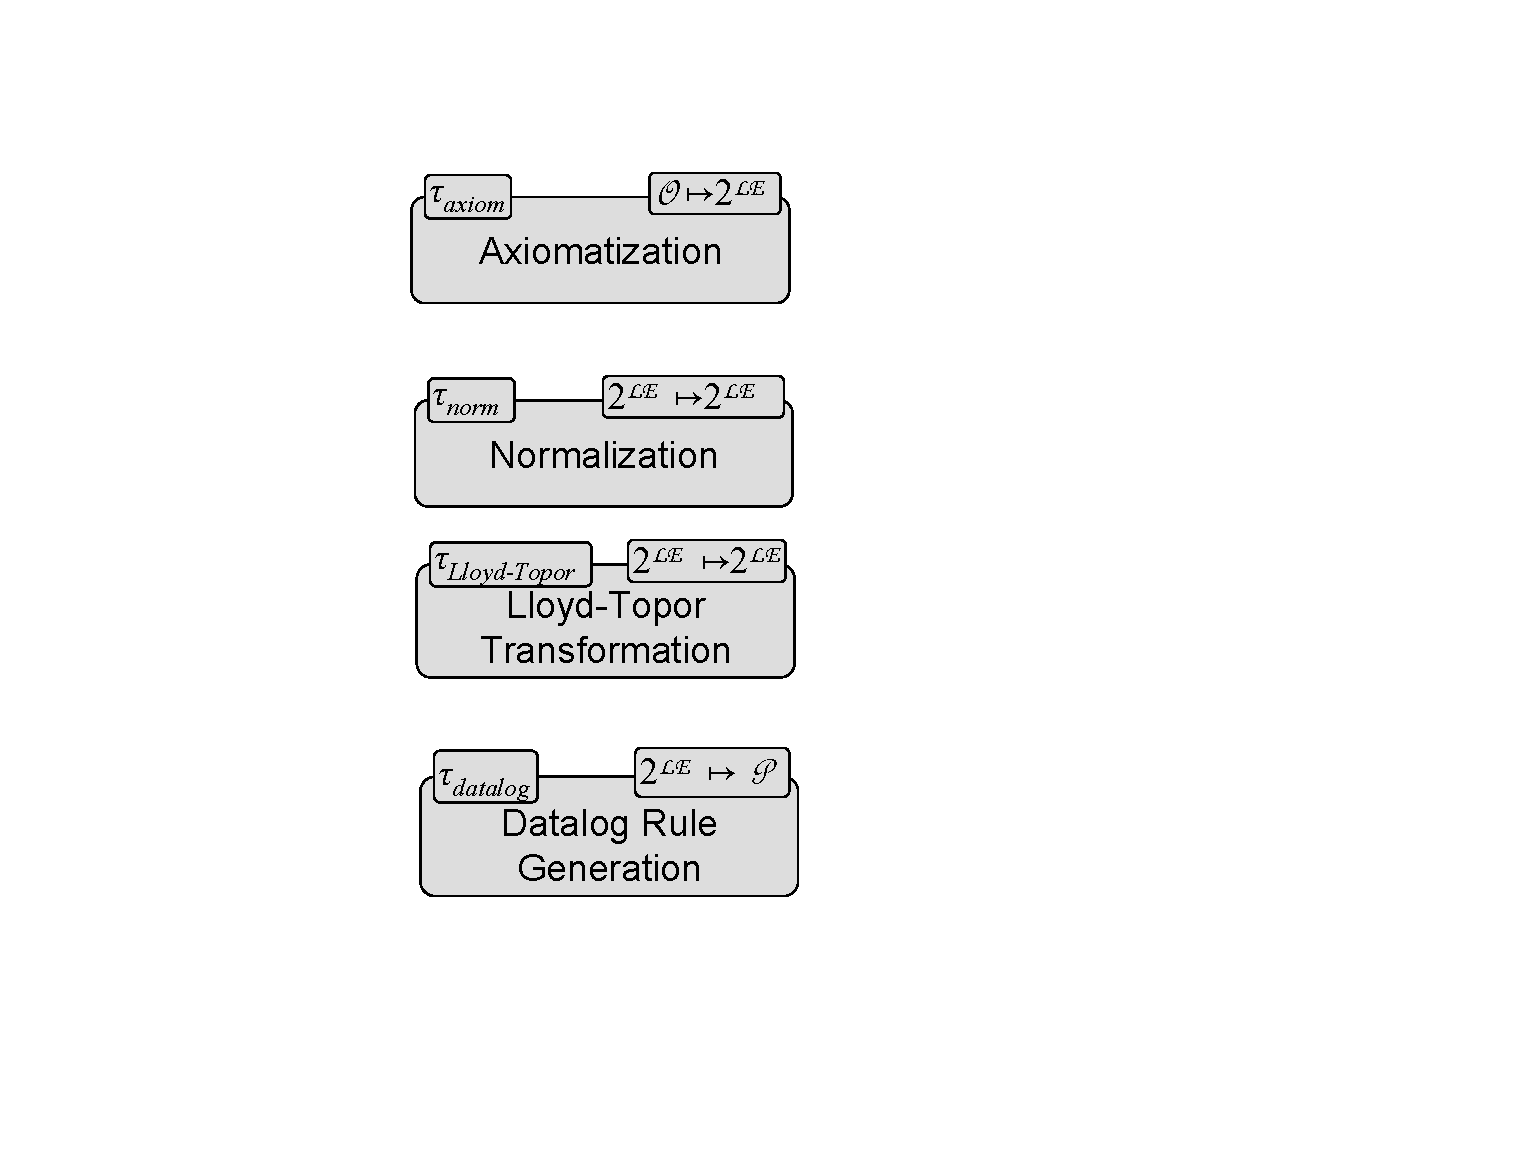
\includegraphics[width=11cm]{figures/layering}
    \centering
    \caption{Internal framework architecture. \label{fig:layering}}
\end{figure}
Figure~\ref{fig:layering} shows the internal architecture of the
framework as well as the data flow during a prototypical usage
scenario. The outer box outlines a WSML reasoner component that
allows a user to register WSML ontologies and to pose queries on
them. The inner box illustrates the transformation pipeline
introduced in Section \ref{sec:mapping} and shows its subsequent
steps in a layering scheme.

Registered ontologies go through all the transformation steps,
whereas user queries are injected at a later stage, skipping the
non-applicable axiomatization and constraint replacement steps.
Here, the internal layering scheme allows for an easy
reorganization and reuse of the transformation steps on demand,
assuring high flexibility and modularity. A good example for this
is the constraint replacement transformation \transdebug: if
included in the pipeline, it produces the rules that activate the
debugging features according to Section \ref{sec:debugging}; if
excluded, the constraints remain in the resulting Datalog program
and are mapped to native constraints of the underlying reasoning
engine.

The core component of the framework is an exchangeable Datalog
inference engine wrapped by a reasoner facade which embeds it in
the framework infrastructure. This facade mediates between the
generic Datalog program produced in the transformations and the
tool-specific Datalog implementation and built-in predicates used
by the external inference engine.

\subsection{Interface and Integration with Existing Technology}
So far we have not detailed on what data structure the framework
operates on. One could implement it directly with a parser and
compiler framework that generates an abstract syntax tree for WSML
which is then directly transformed to the target format (Datalog).
Although this would have performance advantages, it would greatly
reduce reusability and would make maintenance harder. Our framework
is based on an intermediate object model of the language that is
provided by the WSMO4J\footnote{\url{http://wsmo4j.sourceforge.net}}
project. WSMO4J performs the task of parsing and validating WSML
ontologies and provides the source object model for our
translations. In order to enable the usage of different Datalog
engines we additionally implemented a simple object model for
Datalog that is independent from any particular engine. The Datalog
model has objects to represent Literals and Rules, whereas the term
structure is directly reused from WSMO4J (respectively WSML). For
each reasoner that has to be connected to the Framework a small
adapter class has to be written, that is minimally aware of only
Literals, Rules and constants (IRIs) and has to translate them to
the equivalent within the representation of the reasoner. If a
particular reasoner supports additional built-ins and data types
translations for this can iteratively be added.

The WSML reasoner framework currently ships with Facades for two
built-in reasoners: KAON2 and MINS. The initial development was done
with the KAON2 inference engine\footnote{KAON2 is available for
download from \url{http://kaon2.semanticweb.org}}
\cite{hustadt04reducing}. As we have seen in
Section~\ref{sec:datatype_reasoning}, datatype reasoning poses the
biggest challenge for the Datalog implementation. KAON2 provides a
very flexible type system that allows for user-defined datatypes,
together with user-defined predicates on these datatypes, including
type checking predicates. Therefore, KAON2 meets the identified
requirements easily. As a matter of fact, KAON2 already provided
most of the required datatypes and predicates out of the box.

The second reasoner that is currently supported by the framework is
MINS\footnote{\url{http://dev1.deri.at/mins/}}. Whereas KAON2 is the
default reasoner for WSML Flight, MINS can be used for the WSML Rule
variant that includes function symbols and unsafe rules. For
determining which WSML variant a current ontology is in the user of
the framework can use the validation facilities built into
WSMO4J\footnote{A demo of this feature is available at:
\url{http://tools.deri.org/wsml/validator}}.
